\chapter{NUMERICAL SIMULATION SETUP AND RESULTS}

In this section, we introduce our simulation setup, including the directional antenna model, the parameters of the channel and how we generate RSSI samples.
The simulation results will be shown after that.
The simulation code is written in Python.
In the simulation framework, the set up consists of four monitoring devices placed at the corners of the area of interest.
All antennas attached to monitoring devices are pointing towards the center of the area of interest.
The target area is considered to be a square of dimension 6~m~×~6~m inscribed in a larger square of dimension 10~m×10~m.
The two square areas share a same center point.
Again, we use $A_{t}$ to denote the target area, while $A_{o}$ denotes its complement.
We call the inside region the target area, and we refer to its complement as the outside region in the following text.


\section{Antenna Characteristic}

To analyze the effect of radiation characteristics of the sensing antennas on the estimation, isotropic antennas and directional antennas are considered.
The antenna gain of isotropic antennas are zero in all directions.
For the directional antennas, we adopt 3GPP antenna model in~\cite{3GPP-antenna}.
The directional antenna gains obey the following formula,
\begin{equation*}
G_i (\phi_{ij}) = - \min \left\{
12 \left( \frac{\phi_{ij} - \theta_{i}}{\theta_{\mathrm{3dB}}} \right)^2,
G_{\mathrm{floor}} \right\} - G_{\mathrm{avg}}
\end{equation*}
where $\theta_{i}$ is pointing direction of the antenna which is attached to monitoring device~$i$.
Parameter $\theta_{\mathrm{3dB}}$ is the 3~dB beam-width of the radiation pattern.
$G_{floor}$ is a nominal attenuation floor.
$G_{average}$ is a normalization factor, which equal to the average gain over $\in (-180^{\circ}, 180^{\circ}]$,
\begin{equation*}
10 \log_{10} \left( \int_{-180}^{180}
\frac{ 10^{ - \frac{1}{10} \min \left\{
12 \left( \frac{\phi_{ij} - \theta_{i}}{\theta_{\mathrm{3dB}}} \right)^2,
G_{\mathrm{floor}} \right\} } }{360} d \phi_{ij} \right) .
\end{equation*}
The antenna radiation pattern for various 3~dB beam-widths is shown in Fig.~\ref{figure:AntennaCandidates}.
\begin{figure}[t]
	\centerline{\begin{tikzpicture}
\begin{polaraxis}[
%scale only axis,
width=7cm,
xticklabel=$\pgfmathprintnumber{\tick}^\circ$,
y coord trafo/.code=\pgfmathparse{#1+20},
ytick={-16, -8, 0, 8},
ymin=-18, ymax=12,
y coord inv trafo/.code=\pgfmathparse{#1-20},
%height=5cm,
%xlabel={Angle (degree)},
%ylabel={Gain (dB)},
every tick label/.append style={font=\small},
legend entries={\scriptsize{Isotropic},
\scriptsize{$\theta_{\mathrm{3dB}} = 30^{\circ}$},
\scriptsize{$\theta_{\mathrm{3dB}} = 60^{\circ}$},
\scriptsize{$\theta_{\mathrm{3dB}} = 90^{\circ}$},
\scriptsize{$\theta_{\mathrm{3dB}} = 120^{\circ}$}},
legend style={at={(-0.1,0.15)}, nodes=right}
]

% Isotropic
\addplot [
color=black,
densely dotted,
line width=1.5pt
]
coordinates{
(-180, 0) (-179, 0) (-178, 0) (-177, 0)
(-176, 0) (-175, 0) (-174, 0) (-173, 0)
(-172, 0) (-171, 0) (-170, 0) (-169, 0)
(-168, 0) (-167, 0) (-166, 0) (-165, 0)
(-164, 0) (-163, 0) (-162, 0) (-161, 0)
(-160, 0) (-159, 0) (-158, 0) (-157, 0)
(-156, 0) (-155, 0) (-154, 0) (-153, 0)
(-152, 0) (-151, 0) (-150, 0) (-149, 0)
(-148, 0) (-147, 0) (-146, 0) (-145, 0)
(-144, 0) (-143, 0) (-142, 0) (-141, 0)
(-140, 0) (-139, 0) (-138, 0) (-137, 0)
(-136, 0) (-135, 0) (-134, 0) (-133, 0)
(-132, 0) (-131, 0) (-130, 0) (-129, 0)
(-128, 0) (-127, 0) (-126, 0) (-125, 0)
(-124, 0) (-123, 0) (-122, 0) (-121, 0)
(-120, 0) (-119, 0) (-118, 0) (-117, 0)
(-116, 0) (-115, 0) (-114, 0) (-113, 0)
(-112, 0) (-111, 0) (-110, 0) (-109, 0)
(-108, 0) (-107, 0) (-106, 0) (-105, 0)
(-104, 0) (-103, 0) (-102, 0) (-101, 0)
(-100, 0) (-99, 0) (-98, 0) (-97, 0)
(-96, 0) (-95, 0) (-94, 0) (-93, 0)
(-92, 0) (-91, 0) (-90, 0) (-89, 0)
(-88, 0) (-87, 0) (-86, 0) (-85, 0)
(-84, 0) (-83, 0) (-82, 0) (-81, 0)
(-80, 0) (-79, 0) (-78, 0) (-77, 0)
(-76, 0) (-75, 0) (-74, 0) (-73, 0)
(-72, 0) (-71, 0) (-70, 0) (-69, 0)
(-68, 0) (-67, 0) (-66, 0) (-65, 0)
(-64, 0) (-63, 0) (-62, 0) (-61, 0)
(-60, 0) (-59, 0) (-58, 0) (-57, 0)
(-56, 0) (-55, 0) (-54, 0) (-53, 0)
(-52, 0) (-51, 0) (-50, 0) (-49, 0)
(-48, 0) (-47, 0) (-46, 0) (-45, 0)
(-44, 0) (-43, 0) (-42, 0) (-41, 0)
(-40, 0) (-39, 0) (-38, 0) (-37, 0)
(-36, 0) (-35, 0) (-34, 0) (-33, 0)
(-32, 0) (-31, 0) (-30, 0) (-29, 0)
(-28, 0) (-27, 0) (-26, 0) (-25, 0)
(-24, 0) (-23, 0) (-22, 0) (-21, 0)
(-20, 0) (-19, 0) (-18, 0) (-17, 0)
(-16, 0) (-15, 0) (-14, 0) (-13, 0)
(-12, 0) (-11, 0) (-10, 0) ( -9, 0)
( -8, 0) ( -7, 0) ( -6, 0) ( -5, 0)
( -4, 0) ( -3, 0) ( -2, 0) ( -1, 0)
(  0, 0) (  1, 0) (  2, 0) (  3, 0)
(  4, 0) (  5, 0) (  6, 0) (  7, 0)
(  8, 0) (  9, 0) ( 10, 0) ( 11, 0)
( 12, 0) ( 13, 0) ( 14, 0) ( 15, 0)
( 16, 0) ( 17, 0) ( 18, 0) ( 19, 0)
( 20, 0) ( 21, 0) ( 22, 0) ( 23, 0)
( 24, 0) ( 25, 0) ( 26, 0) ( 27, 0)
( 28, 0) ( 29, 0) ( 30, 0) ( 31, 0)
( 32, 0) ( 33, 0) ( 34, 0) ( 35, 0)
( 36, 0) ( 37, 0) ( 38, 0) ( 39, 0)
( 40, 0) ( 41, 0) ( 42, 0) ( 43, 0)
( 44, 0) ( 45, 0) ( 46, 0) ( 47, 0)
( 48, 0) ( 49, 0) ( 50, 0) ( 51, 0)
( 52, 0) ( 53, 0) ( 54, 0) ( 55, 0)
( 56, 0) ( 57, 0) ( 58, 0) ( 59, 0)
( 60, 0) ( 61, 0) ( 62, 0) ( 63, 0)
( 64, 0) ( 65, 0) ( 66, 0) ( 67, 0)
( 68, 0) ( 69, 0) ( 70, 0) ( 71, 0)
( 72, 0) ( 73, 0) ( 74, 0) ( 75, 0)
( 76, 0) ( 77, 0) ( 78, 0) ( 79, 0)
( 80, 0) ( 81, 0) ( 82, 0) ( 83, 0)
( 84, 0) ( 85, 0) ( 86, 0) ( 87, 0)
( 88, 0) ( 89, 0) ( 90, 0) ( 91, 0)
( 92, 0) ( 93, 0) ( 94, 0) ( 95, 0)
( 96, 0) ( 97, 0) ( 98, 0) ( 99, 0)
(100, 0) (101, 0) (102, 0) (103, 0)
(104, 0) (105, 0) (106, 0) (107, 0)
(108, 0) (109, 0) (110, 0) (111, 0)
(112, 0) (113, 0) (114, 0) (115, 0)
(116, 0) (117, 0) (118, 0) (119, 0)
(120, 0) (121, 0) (122, 0) (123, 0)
(124, 0) (125, 0) (126, 0) (127, 0)
(128, 0) (129, 0) (130, 0) (131, 0)
(132, 0) (133, 0) (134, 0) (135, 0)
(136, 0) (137, 0) (138, 0) (139, 0)
(140, 0) (141, 0) (142, 0) (143, 0)
(144, 0) (145, 0) (146, 0) (147, 0)
(148, 0) (149, 0) (150, 0) (151, 0)
(152, 0) (153, 0) (154, 0) (155, 0)
(156, 0) (157, 0) (158, 0) (159, 0)
(160, 0) (161, 0) (162, 0) (163, 0)
(164, 0) (165, 0) (166, 0) (167, 0)
(168, 0) (169, 0) (170, 0) (171, 0)
(172, 0) (173, 0) (174, 0) (175, 0)
(176, 0) (177, 0) (178, 0) (179, 0)
(180, 0)
};

% Theta3dB = 30.0
\addplot [
color=gray,
densely dashed,
line width=1.0pt
]
coordinates{
(-180, -9.8341) (-179, -9.8341) (-178, -9.8341) (-177, -9.8341)
(-176, -9.8341) (-175, -9.8341) (-174, -9.8341) (-173, -9.8341)
(-172, -9.8341) (-171, -9.8341) (-170, -9.8341) (-169, -9.8341)
(-168, -9.8341) (-167, -9.8341) (-166, -9.8341) (-165, -9.8341)
(-164, -9.8341) (-163, -9.8341) (-162, -9.8341) (-161, -9.8341)
(-160, -9.8341) (-159, -9.8341) (-158, -9.8341) (-157, -9.8341)
(-156, -9.8341) (-155, -9.8341) (-154, -9.8341) (-153, -9.8341)
(-152, -9.8341) (-151, -9.8341) (-150, -9.8341) (-149, -9.8341)
(-148, -9.8341) (-147, -9.8341) (-146, -9.8341) (-145, -9.8341)
(-144, -9.8341) (-143, -9.8341) (-142, -9.8341) (-141, -9.8341)
(-140, -9.8341) (-139, -9.8341) (-138, -9.8341) (-137, -9.8341)
(-136, -9.8341) (-135, -9.8341) (-134, -9.8341) (-133, -9.8341)
(-132, -9.8341) (-131, -9.8341) (-130, -9.8341) (-129, -9.8341)
(-128, -9.8341) (-127, -9.8341) (-126, -9.8341) (-125, -9.8341)
(-124, -9.8341) (-123, -9.8341) (-122, -9.8341) (-121, -9.8341)
(-120, -9.8341) (-119, -9.8341) (-118, -9.8341) (-117, -9.8341)
(-116, -9.8341) (-115, -9.8341) (-114, -9.8341) (-113, -9.8341)
(-112, -9.8341) (-111, -9.8341) (-110, -9.8341) (-109, -9.8341)
(-108, -9.8341) (-107, -9.8341) (-106, -9.8341) (-105, -9.8341)
(-104, -9.8341) (-103, -9.8341) (-102, -9.8341) (-101, -9.8341)
(-100, -9.8341) (-99, -9.8341) (-98, -9.8341) (-97, -9.8341)
(-96, -9.8341) (-95, -9.8341) (-94, -9.8341) (-93, -9.8341)
(-92, -9.8341) (-91, -9.8341) (-90, -9.8341) (-89, -9.8341)
(-88, -9.8341) (-87, -9.8341) (-86, -9.8341) (-85, -9.8341)
(-84, -9.8341) (-83, -9.8341) (-82, -9.8341) (-81, -9.8341)
(-80, -9.8341) (-79, -9.8341) (-78, -9.8341) (-77, -9.8341)
(-76, -9.8341) (-75, -9.8341) (-74, -9.8341) (-73, -9.8341)
(-72, -9.8341) (-71, -9.8341) (-70, -9.8341) (-69, -9.8341)
(-68, -9.8341) (-67, -9.8341) (-66, -9.8341) (-65, -9.8341)
(-64, -9.8341) (-63, -9.8341) (-62, -9.8341) (-61, -9.8341)
(-60, -9.8341) (-59, -9.8341) (-58, -9.8341) (-57, -9.8341)
(-56, -9.8341) (-55, -9.8341) (-54, -9.8341) (-53, -9.8341)
(-52, -9.8341) (-51, -9.8341) (-50, -9.8341) (-49, -9.8341)
(-48, -9.8341) (-47, -9.8341) (-46, -9.8341) (-45, -9.8341)
(-44, -9.8341) (-43, -9.8341) (-42, -9.8341) (-41, -9.8341)
(-40, -9.8341) (-39, -9.8341) (-38, -9.0875) (-37, -8.0875)
(-36, -7.1141) (-35, -6.1675) (-34, -5.2475) (-33, -4.3541)
(-32, -3.4875) (-31, -2.6475) (-30, -1.8341) (-29, -1.0475)
(-28, -0.2875) (-27, 0.4459) (-26, 1.1525) (-25, 1.8325)
(-24, 2.4859) (-23, 3.1125) (-22, 3.7125) (-21, 4.2859)
(-20, 4.8325) (-19, 5.3525) (-18, 5.8459) (-17, 6.3125)
(-16, 6.7525) (-15, 7.1659) (-14, 7.5525) (-13, 7.9125)
(-12, 8.2459) (-11, 8.5525) (-10, 8.8325) ( -9, 9.0859)
( -8, 9.3125) ( -7, 9.5125) ( -6, 9.6859) ( -5, 9.8325)
( -4, 9.9525) ( -3, 10.0459) ( -2, 10.1125) ( -1, 10.1525)
(  0, 10.1659) (  1, 10.1525) (  2, 10.1125) (  3, 10.0459)
(  4, 9.9525) (  5, 9.8325) (  6, 9.6859) (  7, 9.5125)
(  8, 9.3125) (  9, 9.0859) ( 10, 8.8325) ( 11, 8.5525)
( 12, 8.2459) ( 13, 7.9125) ( 14, 7.5525) ( 15, 7.1659)
( 16, 6.7525) ( 17, 6.3125) ( 18, 5.8459) ( 19, 5.3525)
( 20, 4.8325) ( 21, 4.2859) ( 22, 3.7125) ( 23, 3.1125)
( 24, 2.4859) ( 25, 1.8325) ( 26, 1.1525) ( 27, 0.4459)
( 28, -0.2875) ( 29, -1.0475) ( 30, -1.8341) ( 31, -2.6475)
( 32, -3.4875) ( 33, -4.3541) ( 34, -5.2475) ( 35, -6.1675)
( 36, -7.1141) ( 37, -8.0875) ( 38, -9.0875) ( 39, -9.8341)
( 40, -9.8341) ( 41, -9.8341) ( 42, -9.8341) ( 43, -9.8341)
( 44, -9.8341) ( 45, -9.8341) ( 46, -9.8341) ( 47, -9.8341)
( 48, -9.8341) ( 49, -9.8341) ( 50, -9.8341) ( 51, -9.8341)
( 52, -9.8341) ( 53, -9.8341) ( 54, -9.8341) ( 55, -9.8341)
( 56, -9.8341) ( 57, -9.8341) ( 58, -9.8341) ( 59, -9.8341)
( 60, -9.8341) ( 61, -9.8341) ( 62, -9.8341) ( 63, -9.8341)
( 64, -9.8341) ( 65, -9.8341) ( 66, -9.8341) ( 67, -9.8341)
( 68, -9.8341) ( 69, -9.8341) ( 70, -9.8341) ( 71, -9.8341)
( 72, -9.8341) ( 73, -9.8341) ( 74, -9.8341) ( 75, -9.8341)
( 76, -9.8341) ( 77, -9.8341) ( 78, -9.8341) ( 79, -9.8341)
( 80, -9.8341) ( 81, -9.8341) ( 82, -9.8341) ( 83, -9.8341)
( 84, -9.8341) ( 85, -9.8341) ( 86, -9.8341) ( 87, -9.8341)
( 88, -9.8341) ( 89, -9.8341) ( 90, -9.8341) ( 91, -9.8341)
( 92, -9.8341) ( 93, -9.8341) ( 94, -9.8341) ( 95, -9.8341)
( 96, -9.8341) ( 97, -9.8341) ( 98, -9.8341) ( 99, -9.8341)
(100, -9.8341) (101, -9.8341) (102, -9.8341) (103, -9.8341)
(104, -9.8341) (105, -9.8341) (106, -9.8341) (107, -9.8341)
(108, -9.8341) (109, -9.8341) (110, -9.8341) (111, -9.8341)
(112, -9.8341) (113, -9.8341) (114, -9.8341) (115, -9.8341)
(116, -9.8341) (117, -9.8341) (118, -9.8341) (119, -9.8341)
(120, -9.8341) (121, -9.8341) (122, -9.8341) (123, -9.8341)
(124, -9.8341) (125, -9.8341) (126, -9.8341) (127, -9.8341)
(128, -9.8341) (129, -9.8341) (130, -9.8341) (131, -9.8341)
(132, -9.8341) (133, -9.8341) (134, -9.8341) (135, -9.8341)
(136, -9.8341) (137, -9.8341) (138, -9.8341) (139, -9.8341)
(140, -9.8341) (141, -9.8341) (142, -9.8341) (143, -9.8341)
(144, -9.8341) (145, -9.8341) (146, -9.8341) (147, -9.8341)
(148, -9.8341) (149, -9.8341) (150, -9.8341) (151, -9.8341)
(152, -9.8341) (153, -9.8341) (154, -9.8341) (155, -9.8341)
(156, -9.8341) (157, -9.8341) (158, -9.8341) (159, -9.8341)
(160, -9.8341) (161, -9.8341) (162, -9.8341) (163, -9.8341)
(164, -9.8341) (165, -9.8341) (166, -9.8341) (167, -9.8341)
(168, -9.8341) (169, -9.8341) (170, -9.8341) (171, -9.8341)
(172, -9.8341) (173, -9.8341) (174, -9.8341) (175, -9.8341)
(176, -9.8341) (177, -9.8341) (178, -9.8341) (179, -9.8341)
(180, -9.8341)
};

% Theta3dB = 60.0
\addplot [
color=gray,
dashed,
line width=1.0pt
]
coordinates{
(-180, -12.6128) (-179, -12.6128) (-178, -12.6128) (-177, -12.6128)
(-176, -12.6128) (-175, -12.6128) (-174, -12.6128) (-173, -12.6128)
(-172, -12.6128) (-171, -12.6128) (-170, -12.6128) (-169, -12.6128)
(-168, -12.6128) (-167, -12.6128) (-166, -12.6128) (-165, -12.6128)
(-164, -12.6128) (-163, -12.6128) (-162, -12.6128) (-161, -12.6128)
(-160, -12.6128) (-159, -12.6128) (-158, -12.6128) (-157, -12.6128)
(-156, -12.6128) (-155, -12.6128) (-154, -12.6128) (-153, -12.6128)
(-152, -12.6128) (-151, -12.6128) (-150, -12.6128) (-149, -12.6128)
(-148, -12.6128) (-147, -12.6128) (-146, -12.6128) (-145, -12.6128)
(-144, -12.6128) (-143, -12.6128) (-142, -12.6128) (-141, -12.6128)
(-140, -12.6128) (-139, -12.6128) (-138, -12.6128) (-137, -12.6128)
(-136, -12.6128) (-135, -12.6128) (-134, -12.6128) (-133, -12.6128)
(-132, -12.6128) (-131, -12.6128) (-130, -12.6128) (-129, -12.6128)
(-128, -12.6128) (-127, -12.6128) (-126, -12.6128) (-125, -12.6128)
(-124, -12.6128) (-123, -12.6128) (-122, -12.6128) (-121, -12.6128)
(-120, -12.6128) (-119, -12.6128) (-118, -12.6128) (-117, -12.6128)
(-116, -12.6128) (-115, -12.6128) (-114, -12.6128) (-113, -12.6128)
(-112, -12.6128) (-111, -12.6128) (-110, -12.6128) (-109, -12.6128)
(-108, -12.6128) (-107, -12.6128) (-106, -12.6128) (-105, -12.6128)
(-104, -12.6128) (-103, -12.6128) (-102, -12.6128) (-101, -12.6128)
(-100, -12.6128) (-99, -12.6128) (-98, -12.6128) (-97, -12.6128)
(-96, -12.6128) (-95, -12.6128) (-94, -12.6128) (-93, -12.6128)
(-92, -12.6128) (-91, -12.6128) (-90, -12.6128) (-89, -12.6128)
(-88, -12.6128) (-87, -12.6128) (-86, -12.6128) (-85, -12.6128)
(-84, -12.6128) (-83, -12.6128) (-82, -12.6128) (-81, -12.6128)
(-80, -12.6128) (-79, -12.6128) (-78, -12.6128) (-77, -12.3761)
(-76, -11.8661) (-75, -11.3628) (-74, -10.8661) (-73, -10.3761)
(-72, -9.8928) (-71, -9.4161) (-70, -8.9461) (-69, -8.4828)
(-68, -8.0261) (-67, -7.5761) (-66, -7.1328) (-65, -6.6961)
(-64, -6.2661) (-63, -5.8428) (-62, -5.4261) (-61, -5.0161)
(-60, -4.6128) (-59, -4.2161) (-58, -3.8261) (-57, -3.4428)
(-56, -3.0661) (-55, -2.6961) (-54, -2.3328) (-53, -1.9761)
(-52, -1.6261) (-51, -1.2828) (-50, -0.9461) (-49, -0.6161)
(-48, -0.2928) (-47, 0.0239) (-46, 0.3339) (-45, 0.6372)
(-44, 0.9339) (-43, 1.2239) (-42, 1.5072) (-41, 1.7839)
(-40, 2.0539) (-39, 2.3172) (-38, 2.5739) (-37, 2.8239)
(-36, 3.0672) (-35, 3.3039) (-34, 3.5339) (-33, 3.7572)
(-32, 3.9739) (-31, 4.1839) (-30, 4.3872) (-29, 4.5839)
(-28, 4.7739) (-27, 4.9572) (-26, 5.1339) (-25, 5.3039)
(-24, 5.4672) (-23, 5.6239) (-22, 5.7739) (-21, 5.9172)
(-20, 6.0539) (-19, 6.1839) (-18, 6.3072) (-17, 6.4239)
(-16, 6.5339) (-15, 6.6372) (-14, 6.7339) (-13, 6.8239)
(-12, 6.9072) (-11, 6.9839) (-10, 7.0539) ( -9, 7.1172)
( -8, 7.1739) ( -7, 7.2239) ( -6, 7.2672) ( -5, 7.3039)
( -4, 7.3339) ( -3, 7.3572) ( -2, 7.3739) ( -1, 7.3839)
(  0, 7.3872) (  1, 7.3839) (  2, 7.3739) (  3, 7.3572)
(  4, 7.3339) (  5, 7.3039) (  6, 7.2672) (  7, 7.2239)
(  8, 7.1739) (  9, 7.1172) ( 10, 7.0539) ( 11, 6.9839)
( 12, 6.9072) ( 13, 6.8239) ( 14, 6.7339) ( 15, 6.6372)
( 16, 6.5339) ( 17, 6.4239) ( 18, 6.3072) ( 19, 6.1839)
( 20, 6.0539) ( 21, 5.9172) ( 22, 5.7739) ( 23, 5.6239)
( 24, 5.4672) ( 25, 5.3039) ( 26, 5.1339) ( 27, 4.9572)
( 28, 4.7739) ( 29, 4.5839) ( 30, 4.3872) ( 31, 4.1839)
( 32, 3.9739) ( 33, 3.7572) ( 34, 3.5339) ( 35, 3.3039)
( 36, 3.0672) ( 37, 2.8239) ( 38, 2.5739) ( 39, 2.3172)
( 40, 2.0539) ( 41, 1.7839) ( 42, 1.5072) ( 43, 1.2239)
( 44, 0.9339) ( 45, 0.6372) ( 46, 0.3339) ( 47, 0.0239)
( 48, -0.2928) ( 49, -0.6161) ( 50, -0.9461) ( 51, -1.2828)
( 52, -1.6261) ( 53, -1.9761) ( 54, -2.3328) ( 55, -2.6961)
( 56, -3.0661) ( 57, -3.4428) ( 58, -3.8261) ( 59, -4.2161)
( 60, -4.6128) ( 61, -5.0161) ( 62, -5.4261) ( 63, -5.8428)
( 64, -6.2661) ( 65, -6.6961) ( 66, -7.1328) ( 67, -7.5761)
( 68, -8.0261) ( 69, -8.4828) ( 70, -8.9461) ( 71, -9.4161)
( 72, -9.8928) ( 73, -10.3761) ( 74, -10.8661) ( 75, -11.3628)
( 76, -11.8661) ( 77, -12.3761) ( 78, -12.6128) ( 79, -12.6128)
( 80, -12.6128) ( 81, -12.6128) ( 82, -12.6128) ( 83, -12.6128)
( 84, -12.6128) ( 85, -12.6128) ( 86, -12.6128) ( 87, -12.6128)
( 88, -12.6128) ( 89, -12.6128) ( 90, -12.6128) ( 91, -12.6128)
( 92, -12.6128) ( 93, -12.6128) ( 94, -12.6128) ( 95, -12.6128)
( 96, -12.6128) ( 97, -12.6128) ( 98, -12.6128) ( 99, -12.6128)
(100, -12.6128) (101, -12.6128) (102, -12.6128) (103, -12.6128)
(104, -12.6128) (105, -12.6128) (106, -12.6128) (107, -12.6128)
(108, -12.6128) (109, -12.6128) (110, -12.6128) (111, -12.6128)
(112, -12.6128) (113, -12.6128) (114, -12.6128) (115, -12.6128)
(116, -12.6128) (117, -12.6128) (118, -12.6128) (119, -12.6128)
(120, -12.6128) (121, -12.6128) (122, -12.6128) (123, -12.6128)
(124, -12.6128) (125, -12.6128) (126, -12.6128) (127, -12.6128)
(128, -12.6128) (129, -12.6128) (130, -12.6128) (131, -12.6128)
(132, -12.6128) (133, -12.6128) (134, -12.6128) (135, -12.6128)
(136, -12.6128) (137, -12.6128) (138, -12.6128) (139, -12.6128)
(140, -12.6128) (141, -12.6128) (142, -12.6128) (143, -12.6128)
(144, -12.6128) (145, -12.6128) (146, -12.6128) (147, -12.6128)
(148, -12.6128) (149, -12.6128) (150, -12.6128) (151, -12.6128)
(152, -12.6128) (153, -12.6128) (154, -12.6128) (155, -12.6128)
(156, -12.6128) (157, -12.6128) (158, -12.6128) (159, -12.6128)
(160, -12.6128) (161, -12.6128) (162, -12.6128) (163, -12.6128)
(164, -12.6128) (165, -12.6128) (166, -12.6128) (167, -12.6128)
(168, -12.6128) (169, -12.6128) (170, -12.6128) (171, -12.6128)
(172, -12.6128) (173, -12.6128) (174, -12.6128) (175, -12.6128)
(176, -12.6128) (177, -12.6128) (178, -12.6128) (179, -12.6128)
(180, -12.6128)
};

% Theta3dB = 90.0
\addplot [
color=black,
solid,
line width=1.5pt
]
coordinates{
(-180, -14.2936) (-179, -14.2936) (-178, -14.2936) (-177, -14.2936)
(-176, -14.2936) (-175, -14.2936) (-174, -14.2936) (-173, -14.2936)
(-172, -14.2936) (-171, -14.2936) (-170, -14.2936) (-169, -14.2936)
(-168, -14.2936) (-167, -14.2936) (-166, -14.2936) (-165, -14.2936)
(-164, -14.2936) (-163, -14.2936) (-162, -14.2936) (-161, -14.2936)
(-160, -14.2936) (-159, -14.2936) (-158, -14.2936) (-157, -14.2936)
(-156, -14.2936) (-155, -14.2936) (-154, -14.2936) (-153, -14.2936)
(-152, -14.2936) (-151, -14.2936) (-150, -14.2936) (-149, -14.2936)
(-148, -14.2936) (-147, -14.2936) (-146, -14.2936) (-145, -14.2936)
(-144, -14.2936) (-143, -14.2936) (-142, -14.2936) (-141, -14.2936)
(-140, -14.2936) (-139, -14.2936) (-138, -14.2936) (-137, -14.2936)
(-136, -14.2936) (-135, -14.2936) (-134, -14.2936) (-133, -14.2936)
(-132, -14.2936) (-131, -14.2936) (-130, -14.2936) (-129, -14.2936)
(-128, -14.2936) (-127, -14.2936) (-126, -14.2936) (-125, -14.2936)
(-124, -14.2936) (-123, -14.2936) (-122, -14.2936) (-121, -14.2936)
(-120, -14.2936) (-119, -14.2936) (-118, -14.2936) (-117, -14.2936)
(-116, -14.2284) (-115, -13.8862) (-114, -13.5469) (-113, -13.2106)
(-112, -12.8773) (-111, -12.5469) (-110, -12.2195) (-109, -11.8951)
(-108, -11.5736) (-107, -11.2551) (-106, -10.9395) (-105, -10.6269)
(-104, -10.3173) (-103, -10.0106) (-102, -9.7069) (-101, -9.4062)
(-100, -9.1084) (-99, -8.8136) (-98, -8.5218) (-97, -8.2329)
(-96, -7.9469) (-95, -7.6640) (-94, -7.3840) (-93, -7.1069)
(-92, -6.8329) (-91, -6.5618) (-90, -6.2936) (-89, -6.0284)
(-88, -5.7662) (-87, -5.5069) (-86, -5.2506) (-85, -4.9973)
(-84, -4.7469) (-83, -4.4995) (-82, -4.2551) (-81, -4.0136)
(-80, -3.7751) (-79, -3.5395) (-78, -3.3069) (-77, -3.0773)
(-76, -2.8506) (-75, -2.6269) (-74, -2.4062) (-73, -2.1884)
(-72, -1.9736) (-71, -1.7618) (-70, -1.5529) (-69, -1.3469)
(-68, -1.1440) (-67, -0.9440) (-66, -0.7469) (-65, -0.5529)
(-64, -0.3618) (-63, -0.1736) (-62, 0.0116) (-61, 0.1938)
(-60, 0.3731) (-59, 0.5494) (-58, 0.7227) (-57, 0.8931)
(-56, 1.0605) (-55, 1.2249) (-54, 1.3864) (-53, 1.5449)
(-52, 1.7005) (-51, 1.8531) (-50, 2.0027) (-49, 2.1494)
(-48, 2.2931) (-47, 2.4338) (-46, 2.5716) (-45, 2.7064)
(-44, 2.8382) (-43, 2.9671) (-42, 3.0931) (-41, 3.2160)
(-40, 3.3360) (-39, 3.4531) (-38, 3.5671) (-37, 3.6782)
(-36, 3.7864) (-35, 3.8916) (-34, 3.9938) (-33, 4.0931)
(-32, 4.1894) (-31, 4.2827) (-30, 4.3731) (-29, 4.4605)
(-28, 4.5449) (-27, 4.6264) (-26, 4.7049) (-25, 4.7805)
(-24, 4.8531) (-23, 4.9227) (-22, 4.9894) (-21, 5.0531)
(-20, 5.1138) (-19, 5.1716) (-18, 5.2264) (-17, 5.2782)
(-16, 5.3271) (-15, 5.3731) (-14, 5.4160) (-13, 5.4560)
(-12, 5.4931) (-11, 5.5271) (-10, 5.5582) ( -9, 5.5864)
( -8, 5.6116) ( -7, 5.6338) ( -6, 5.6531) ( -5, 5.6694)
( -4, 5.6827) ( -3, 5.6931) ( -2, 5.7005) ( -1, 5.7049)
(  0, 5.7064) (  1, 5.7049) (  2, 5.7005) (  3, 5.6931)
(  4, 5.6827) (  5, 5.6694) (  6, 5.6531) (  7, 5.6338)
(  8, 5.6116) (  9, 5.5864) ( 10, 5.5582) ( 11, 5.5271)
( 12, 5.4931) ( 13, 5.4560) ( 14, 5.4160) ( 15, 5.3731)
( 16, 5.3271) ( 17, 5.2782) ( 18, 5.2264) ( 19, 5.1716)
( 20, 5.1138) ( 21, 5.0531) ( 22, 4.9894) ( 23, 4.9227)
( 24, 4.8531) ( 25, 4.7805) ( 26, 4.7049) ( 27, 4.6264)
( 28, 4.5449) ( 29, 4.4605) ( 30, 4.3731) ( 31, 4.2827)
( 32, 4.1894) ( 33, 4.0931) ( 34, 3.9938) ( 35, 3.8916)
( 36, 3.7864) ( 37, 3.6782) ( 38, 3.5671) ( 39, 3.4531)
( 40, 3.3360) ( 41, 3.2160) ( 42, 3.0931) ( 43, 2.9671)
( 44, 2.8382) ( 45, 2.7064) ( 46, 2.5716) ( 47, 2.4338)
( 48, 2.2931) ( 49, 2.1494) ( 50, 2.0027) ( 51, 1.8531)
( 52, 1.7005) ( 53, 1.5449) ( 54, 1.3864) ( 55, 1.2249)
( 56, 1.0605) ( 57, 0.8931) ( 58, 0.7227) ( 59, 0.5494)
( 60, 0.3731) ( 61, 0.1938) ( 62, 0.0116) ( 63, -0.1736)
( 64, -0.3618) ( 65, -0.5529) ( 66, -0.7469) ( 67, -0.9440)
( 68, -1.1440) ( 69, -1.3469) ( 70, -1.5529) ( 71, -1.7618)
( 72, -1.9736) ( 73, -2.1884) ( 74, -2.4062) ( 75, -2.6269)
( 76, -2.8506) ( 77, -3.0773) ( 78, -3.3069) ( 79, -3.5395)
( 80, -3.7751) ( 81, -4.0136) ( 82, -4.2551) ( 83, -4.4995)
( 84, -4.7469) ( 85, -4.9973) ( 86, -5.2506) ( 87, -5.5069)
( 88, -5.7662) ( 89, -6.0284) ( 90, -6.2936) ( 91, -6.5618)
( 92, -6.8329) ( 93, -7.1069) ( 94, -7.3840) ( 95, -7.6640)
( 96, -7.9469) ( 97, -8.2329) ( 98, -8.5218) ( 99, -8.8136)
(100, -9.1084) (101, -9.4062) (102, -9.7069) (103, -10.0106)
(104, -10.3173) (105, -10.6269) (106, -10.9395) (107, -11.2551)
(108, -11.5736) (109, -11.8951) (110, -12.2195) (111, -12.5469)
(112, -12.8773) (113, -13.2106) (114, -13.5469) (115, -13.8862)
(116, -14.2284) (117, -14.2936) (118, -14.2936) (119, -14.2936)
(120, -14.2936) (121, -14.2936) (122, -14.2936) (123, -14.2936)
(124, -14.2936) (125, -14.2936) (126, -14.2936) (127, -14.2936)
(128, -14.2936) (129, -14.2936) (130, -14.2936) (131, -14.2936)
(132, -14.2936) (133, -14.2936) (134, -14.2936) (135, -14.2936)
(136, -14.2936) (137, -14.2936) (138, -14.2936) (139, -14.2936)
(140, -14.2936) (141, -14.2936) (142, -14.2936) (143, -14.2936)
(144, -14.2936) (145, -14.2936) (146, -14.2936) (147, -14.2936)
(148, -14.2936) (149, -14.2936) (150, -14.2936) (151, -14.2936)
(152, -14.2936) (153, -14.2936) (154, -14.2936) (155, -14.2936)
(156, -14.2936) (157, -14.2936) (158, -14.2936) (159, -14.2936)
(160, -14.2936) (161, -14.2936) (162, -14.2936) (163, -14.2936)
(164, -14.2936) (165, -14.2936) (166, -14.2936) (167, -14.2936)
(168, -14.2936) (169, -14.2936) (170, -14.2936) (171, -14.2936)
(172, -14.2936) (173, -14.2936) (174, -14.2936) (175, -14.2936)
(176, -14.2936) (177, -14.2936) (178, -14.2936) (179, -14.2936)
(180, -14.2936)
};

% Theta3dB = 120.0
\addplot [
color=gray,
dashdotted,
line width=1.0pt
]
coordinates{
(-180, -15.5024) (-179, -15.5024) (-178, -15.5024) (-177, -15.5024)
(-176, -15.5024) (-175, -15.5024) (-174, -15.5024) (-173, -15.5024)
(-172, -15.5024) (-171, -15.5024) (-170, -15.5024) (-169, -15.5024)
(-168, -15.5024) (-167, -15.5024) (-166, -15.5024) (-165, -15.5024)
(-164, -15.5024) (-163, -15.5024) (-162, -15.5024) (-161, -15.5024)
(-160, -15.5024) (-159, -15.5024) (-158, -15.5024) (-157, -15.5024)
(-156, -15.5024) (-155, -15.5024) (-154, -15.2657) (-153, -15.0099)
(-152, -14.7557) (-151, -14.5032) (-150, -14.2524) (-149, -14.0032)
(-148, -13.7557) (-147, -13.5099) (-146, -13.2657) (-145, -13.0232)
(-144, -12.7824) (-143, -12.5432) (-142, -12.3057) (-141, -12.0699)
(-140, -11.8357) (-139, -11.6032) (-138, -11.3724) (-137, -11.1432)
(-136, -10.9157) (-135, -10.6899) (-134, -10.4657) (-133, -10.2432)
(-132, -10.0224) (-131, -9.8032) (-130, -9.5857) (-129, -9.3699)
(-128, -9.1557) (-127, -8.9432) (-126, -8.7324) (-125, -8.5232)
(-124, -8.3157) (-123, -8.1099) (-122, -7.9057) (-121, -7.7032)
(-120, -7.5024) (-119, -7.3032) (-118, -7.1057) (-117, -6.9099)
(-116, -6.7157) (-115, -6.5232) (-114, -6.3324) (-113, -6.1432)
(-112, -5.9557) (-111, -5.7699) (-110, -5.5857) (-109, -5.4032)
(-108, -5.2224) (-107, -5.0432) (-106, -4.8657) (-105, -4.6899)
(-104, -4.5157) (-103, -4.3432) (-102, -4.1724) (-101, -4.0032)
(-100, -3.8357) (-99, -3.6699) (-98, -3.5057) (-97, -3.3432)
(-96, -3.1824) (-95, -3.0232) (-94, -2.8657) (-93, -2.7099)
(-92, -2.5557) (-91, -2.4032) (-90, -2.2524) (-89, -2.1032)
(-88, -1.9557) (-87, -1.8099) (-86, -1.6657) (-85, -1.5232)
(-84, -1.3824) (-83, -1.2432) (-82, -1.1057) (-81, -0.9699)
(-80, -0.8357) (-79, -0.7032) (-78, -0.5724) (-77, -0.4432)
(-76, -0.3157) (-75, -0.1899) (-74, -0.0657) (-73, 0.0568)
(-72, 0.1776) (-71, 0.2968) (-70, 0.4143) (-69, 0.5301)
(-68, 0.6443) (-67, 0.7568) (-66, 0.8676) (-65, 0.9768)
(-64, 1.0843) (-63, 1.1901) (-62, 1.2943) (-61, 1.3968)
(-60, 1.4976) (-59, 1.5968) (-58, 1.6943) (-57, 1.7901)
(-56, 1.8843) (-55, 1.9768) (-54, 2.0676) (-53, 2.1568)
(-52, 2.2443) (-51, 2.3301) (-50, 2.4143) (-49, 2.4968)
(-48, 2.5776) (-47, 2.6568) (-46, 2.7343) (-45, 2.8101)
(-44, 2.8843) (-43, 2.9568) (-42, 3.0276) (-41, 3.0968)
(-40, 3.1643) (-39, 3.2301) (-38, 3.2943) (-37, 3.3568)
(-36, 3.4176) (-35, 3.4768) (-34, 3.5343) (-33, 3.5901)
(-32, 3.6443) (-31, 3.6968) (-30, 3.7476) (-29, 3.7968)
(-28, 3.8443) (-27, 3.8901) (-26, 3.9343) (-25, 3.9768)
(-24, 4.0176) (-23, 4.0568) (-22, 4.0943) (-21, 4.1301)
(-20, 4.1643) (-19, 4.1968) (-18, 4.2276) (-17, 4.2568)
(-16, 4.2843) (-15, 4.3101) (-14, 4.3343) (-13, 4.3568)
(-12, 4.3776) (-11, 4.3968) (-10, 4.4143) ( -9, 4.4301)
( -8, 4.4443) ( -7, 4.4568) ( -6, 4.4676) ( -5, 4.4768)
( -4, 4.4843) ( -3, 4.4901) ( -2, 4.4943) ( -1, 4.4968)
(  0, 4.4976) (  1, 4.4968) (  2, 4.4943) (  3, 4.4901)
(  4, 4.4843) (  5, 4.4768) (  6, 4.4676) (  7, 4.4568)
(  8, 4.4443) (  9, 4.4301) ( 10, 4.4143) ( 11, 4.3968)
( 12, 4.3776) ( 13, 4.3568) ( 14, 4.3343) ( 15, 4.3101)
( 16, 4.2843) ( 17, 4.2568) ( 18, 4.2276) ( 19, 4.1968)
( 20, 4.1643) ( 21, 4.1301) ( 22, 4.0943) ( 23, 4.0568)
( 24, 4.0176) ( 25, 3.9768) ( 26, 3.9343) ( 27, 3.8901)
( 28, 3.8443) ( 29, 3.7968) ( 30, 3.7476) ( 31, 3.6968)
( 32, 3.6443) ( 33, 3.5901) ( 34, 3.5343) ( 35, 3.4768)
( 36, 3.4176) ( 37, 3.3568) ( 38, 3.2943) ( 39, 3.2301)
( 40, 3.1643) ( 41, 3.0968) ( 42, 3.0276) ( 43, 2.9568)
( 44, 2.8843) ( 45, 2.8101) ( 46, 2.7343) ( 47, 2.6568)
( 48, 2.5776) ( 49, 2.4968) ( 50, 2.4143) ( 51, 2.3301)
( 52, 2.2443) ( 53, 2.1568) ( 54, 2.0676) ( 55, 1.9768)
( 56, 1.8843) ( 57, 1.7901) ( 58, 1.6943) ( 59, 1.5968)
( 60, 1.4976) ( 61, 1.3968) ( 62, 1.2943) ( 63, 1.1901)
( 64, 1.0843) ( 65, 0.9768) ( 66, 0.8676) ( 67, 0.7568)
( 68, 0.6443) ( 69, 0.5301) ( 70, 0.4143) ( 71, 0.2968)
( 72, 0.1776) ( 73, 0.0568) ( 74, -0.0657) ( 75, -0.1899)
( 76, -0.3157) ( 77, -0.4432) ( 78, -0.5724) ( 79, -0.7032)
( 80, -0.8357) ( 81, -0.9699) ( 82, -1.1057) ( 83, -1.2432)
( 84, -1.3824) ( 85, -1.5232) ( 86, -1.6657) ( 87, -1.8099)
( 88, -1.9557) ( 89, -2.1032) ( 90, -2.2524) ( 91, -2.4032)
( 92, -2.5557) ( 93, -2.7099) ( 94, -2.8657) ( 95, -3.0232)
( 96, -3.1824) ( 97, -3.3432) ( 98, -3.5057) ( 99, -3.6699)
(100, -3.8357) (101, -4.0032) (102, -4.1724) (103, -4.3432)
(104, -4.5157) (105, -4.6899) (106, -4.8657) (107, -5.0432)
(108, -5.2224) (109, -5.4032) (110, -5.5857) (111, -5.7699)
(112, -5.9557) (113, -6.1432) (114, -6.3324) (115, -6.5232)
(116, -6.7157) (117, -6.9099) (118, -7.1057) (119, -7.3032)
(120, -7.5024) (121, -7.7032) (122, -7.9057) (123, -8.1099)
(124, -8.3157) (125, -8.5232) (126, -8.7324) (127, -8.9432)
(128, -9.1557) (129, -9.3699) (130, -9.5857) (131, -9.8032)
(132, -10.0224) (133, -10.2432) (134, -10.4657) (135, -10.6899)
(136, -10.9157) (137, -11.1432) (138, -11.3724) (139, -11.6032)
(140, -11.8357) (141, -12.0699) (142, -12.3057) (143, -12.5432)
(144, -12.7824) (145, -13.0232) (146, -13.2657) (147, -13.5099)
(148, -13.7557) (149, -14.0032) (150, -14.2524) (151, -14.5032)
(152, -14.7557) (153, -15.0099) (154, -15.2657) (155, -15.5024)
(156, -15.5024) (157, -15.5024) (158, -15.5024) (159, -15.5024)
(160, -15.5024) (161, -15.5024) (162, -15.5024) (163, -15.5024)
(164, -15.5024) (165, -15.5024) (166, -15.5024) (167, -15.5024)
(168, -15.5024) (169, -15.5024) (170, -15.5024) (171, -15.5024)
(172, -15.5024) (173, -15.5024) (174, -15.5024) (175, -15.5024)
(176, -15.5024) (177, -15.5024) (178, -15.5024) (179, -15.5024)
(180, -15.5024)
};

\end{polaraxis}
\end{tikzpicture}

}
	\caption{This graph depicts normalized antenna radiation patterns. The pointing direction is set to $ 0^{\circ}$ and $G_{\mathrm{floor}} = 20~\mathrm{dB}$.}
	\label{figure:AntennaCandidates}
\end{figure}


\section{Channel Characteristic}

As mentioned in Chapter~\ref{chapter:SystemModel}, the channel model we adopt is the log-normal path loss model.
The received signal power can be expressed as
\begin{equation} \label{equation:Power}
P \text{[dBm]}
= A + B \log_{10}(d) + L + G (\phi) .
\end{equation}
In this equation, the physical parameters are based on regulation issued by the Federal Communications Commission (FCC) and on the profiles of typical wireless environments.
According to the Friis transmission equation~\cite{friis1946note}, we have
\begin{equation*}
A = P_{\mathrm{t}} + 20 \log_{10} \left( \frac{3 \times 10^8}{f_{\mathrm{carrier}}} \right) - 20\log_{10}(4\pi) 
\end{equation*}
where $P_{t}$ is the mobile devices transmission power, which is set to 20~dBm.
The frequency $f_{carrier}$ is that of the Wi-Fi signal wave, 2.462~GHz~\cite{goldsmith2005wireless}.
Accordingly, $A$ is equal to $-20.27$~dBm.
We set the path-loss parameter $B$ to -20~dBm, which is the coefficient associated with free-space.
The logarithmic $\sigma_{s}$, which represents variation in shadow fading, is set to 2.0~dBm.


\section{Generating Data Set}

As mentioned above, the inference task is based on the received power matrix, which is collected by the monitoring devices.
In the simulation, we generate the sample data according to the antenna gain model and the channel model discussed above.
The parameter values we use to create the data set are summarized in Table~\ref{table:PhysicalParameters}.
\begin{table}[bht]
	\caption{System parameters used during simulations.} \label{table:PhysicalParameters}
	\centerline{
		\begin{tabular}{|l|l|}
			\hline
			\multicolumn{1}{|c|}{\textbf{Physical Parameters}} &
			\multicolumn{1}{|c|}{\textbf{Values}} \\
			\hline
			Nominal Power & $A = -20.27$~dBm \\
			\hline
			Free-Space Loss parameter & $B = - 20$~dBm \\
			\hline
			Logarithmic Standard Deviation & $\sigma_{\mathrm{s}} = 2.0$~dBm \\
			\hline
			3~dB Beam-width (directional) & $\theta_{\mathrm{3dB}} = 90^{\circ}$ \\
			\hline
			Antenna Floor & $G_{\mathrm{floor}} = 20$~dB \\
			\hline
		\end{tabular}}
\end{table}
We generate the numerical data set as follow.
We denote the location of the four monitoring devices as $\{ \mathbf{s}_i \}$ $i \in{1,2,3,4}$.
First, we set a certain value $\lambda$, which represents the aggregate Poisson rate across the two monitored regions (inside region and outside region) equal to 32.
The splitting parameter between two regions is $\alpha$.
Thus,
\begin{xalignat*}{2}
	\lambda_{\mathrm{t}}
	&= \alpha \frac{\lambda}{A_{\mathrm{t}}}
	&\lambda_{\mathrm{o}}
	&= (1 - \alpha) \frac{\lambda}{A_{\mathrm{o}}}
\end{xalignat*}
where $\lambda_{t}$ is the Poisson rate of inside region and $\lambda_{o}$ is the Poisson rate of outside region.
Once $\lambda_{t}$ and $\lambda_{o}$ are determined, $r_{t}$ the number of devices inside and $r_{o}$ the number of devices outside are established using Poisson trials,
\begin{xalignat*}{2}
	R_{\mathrm{t}} &\sim
	\frac{\left( A_{\mathrm{t}} \lambda_{\mathrm{t}} \right)^k}{k!}
	e^{- A_{\mathrm{t}} \lambda_{\mathrm{t}}}
	&R_{\mathrm{o}} &\sim
	\frac{\left( A_{\mathrm{o}} \lambda_{\mathrm{o}} \right)^k}{k!}
	e^{- A_{\mathrm{o}} \lambda_{\mathrm{o}}} .
\end{xalignat*}
Each of $R_{{t}} = r_{{t}}$ devices inside the target area is independently assigned a location according to a uniform distribution.
Likewise, each of $R_{\mathrm{o}} = r_{\mathrm{o}}$ devices outside is independently assigned a location according to another uniform distribution.
Therefore, we obtain the location vector $\underline{\mathbf{U}} = \underline{\mathbf{u}}$ of the wireless clients.
For each of the wireless clients, a collection of four received signal strength corresponding to the four monitoring devices is computed according to \eqref{equation:Power}.
The shadow fading component $L$ is generated following a log-normal distribution whose standard deviation $\sigma_{s}=2.0$~dBm.
Finally, we get the sequence of power vectors $\underline{\mathbf{p}} = (\mathbf{p}_1, \ldots, \mathbf{p}_{n_{\mathrm{a}}})$, where vector $\mathbf{p}_j$ corresponding to wireless client $j$ contains four power strength received by four monitoring devices respectively.


\section{Performance Analysis}

The proposed estimators act on observation vector $\mathbf{p}$


\subsection{Bayes Estimation}

We first consider the performance of the Bayes estimation framework introduced in Section~\ref{section:BayesEstimation}.
As is discussed in the previous section, the Poisson rate of the combined two regions $\lambda$, the Poisson rate of inside region $\lambda_{t}$ and the Poisson rate of outside region $\lambda_{o}$ have the following relation along with the splitting parameter $\alpha$,
\begin{xalignat*}{2}
	\lambda_{\mathrm{t}}
	&= \alpha \frac{\lambda}{A_{\mathrm{t}}}
	&\lambda_{\mathrm{o}}
	&= (1 - \alpha) \frac{\lambda}{A_{\mathrm{o}}} .
\end{xalignat*}
In the simulation results, the area of inside region $A_{t}$ is equal to 36, and the area of outside region $A_{o}$ is equal to 64.
We can plot performance results as a function of the splitting coefficient $\alpha$.
The vertical axis represents the BMSE of Bayes estimator.
The black curve in Fig.~\ref{figure: BayesRt} shows the BMSE when the Bayes estimator operates on data collected using isotropic antennas.
The red curve in Fig.~\ref{figure: BayesRt} corresponds to four directional antennas located at the four corners of the target area and pointing directly to the center.
These antennas have a 3~dB beam-width of $\theta_{\mathrm{3dB}} = 90^{\circ}$ and a nominal attenuation floor of $G_{\mathrm{floor}} = 20$~dB.
Every point is obtained by averaging over fifty thousand trials.
\begin{figure}[]
	\centering
	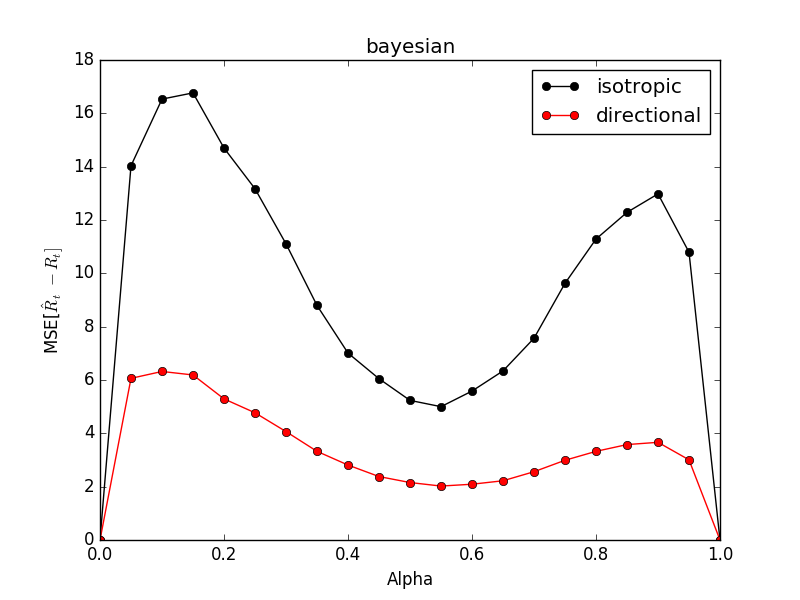
\includegraphics[scale=0.6]{Figures/bayesRt.png}
	\caption{This graph shows Bayesian mean squared error as functions of splitting parameter under scheme of \ref{section:BayesEstimation}. Black line correspond to performance of system equipped with isotropic antennas, whereas red line correspond to the performance of systems with directional antennas. }
	\label{figure: BayesRt}
\end{figure}
According to Fig.~\ref{figure: BayesRt}, systems with directional antennas perform better than systems with isotropic antennas.

To further compare the performances, we introduce confidence intervals.
A confidence level refers to the percentage of all possible samples that can be expected to include the true population parameter~\cite{altman2013statistics}.
Suppose we use the same sampling method to select different samples and to compute a different interval estimate for each sample.
Some interval estimates would include the true population parameter and some may not.
A 95\% confidence level means that 95\% of the intervals would include the true parameter.
Generally, the confidence interval is computed as below.
Select a confidence level which describes the uncertainty of a sampling method.
Compute $\alpha$,
\begin{equation*}
\alpha = 1 - (\text{confidence level} / 100) .
\end{equation*}
Find the critical probability $p^*$
\begin{equation*}
p^* = 1 - \alpha/2 .
\end{equation*}
Express the critical value as a $t$-statistic by using degree of freedom and critical probability, where degree of freedom equals to
\begin{equation*}
df = N-1
\end{equation*}
and $N$ is the sample size.
The standard error $SE$ is given as
\begin{equation*}
SE= \dfrac{\sigma}{\sqrt{N}}
\end{equation*}
where $\sigma$ is the standard deviation of the sample.
The magin of error is the product of critical value $t^*$ and $SE$.
The confidence interval is expressed as
\begin{equation*}
\text{Confidence interval} = \mu \pm \text{Margin of error}
\end{equation*}
where $\mu$ is the mean of the sample.
In this simulation, we analyze the absolute difference between the real number of active devices inside $r_{t}$ and the estimator result $\hat{r_{t}}$.
The confidence intervals of $|r_{t}-\hat{r_{t}}|$ corresponding to isotropic antennas and directional antennas are summarized in Table~\ref{table:ConfidenceBayes}.
The result is based on fifty thousand samples.
\begin{table}[bht]
	\caption{Confidence interval of $|r_{t}-\hat{r_{t}}|$ for simulation Bayes scheme} \label{table:ConfidenceBayes}
	\centerline{
		\begin{tabular}{|l|l|}
			\hline
			\multicolumn{1}{|c|}{\textbf{Antenna type}} &
			\multicolumn{1}{|c|}{\textbf{Confidence interval}} \\
			\hline
			Directional & $1.412411 \pm 0.002166$ \\
			\hline
			Isotropic & $2.454623 \pm 0.003450$ \\
			\hline
		\end{tabular}}
	\end{table}
To make the result more straightforward, we use Gaussian kernel density estimation to plot the approximation of the probability density function of $|r_{t}-\hat{r_{t}}|$.
The horizontal axis represents value for $|r_{t}-\hat{r_{t}}|$.
\begin{figure}[]
	\centering
	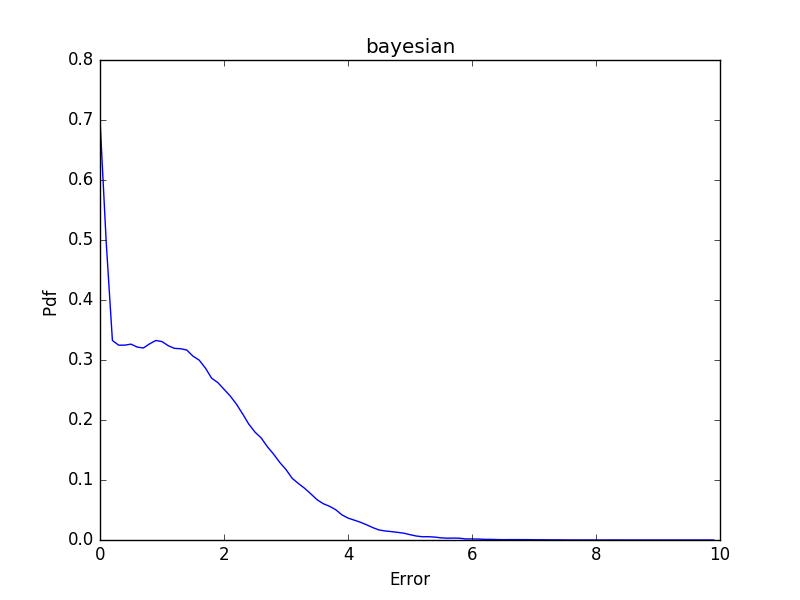
\includegraphics[scale=0.5]{Figures/bayesrtdir.png}
	\caption{This graph shows the approximation probability density function of $|r_{t}-\hat{r_{t}}|$ corresponding to system equipped with directional antennas under the scheme of Section~\ref{section:BayesEstimation}. }
	\label{figure: BayesRtdir}
\end{figure}
\begin{figure}[]
	\centering
	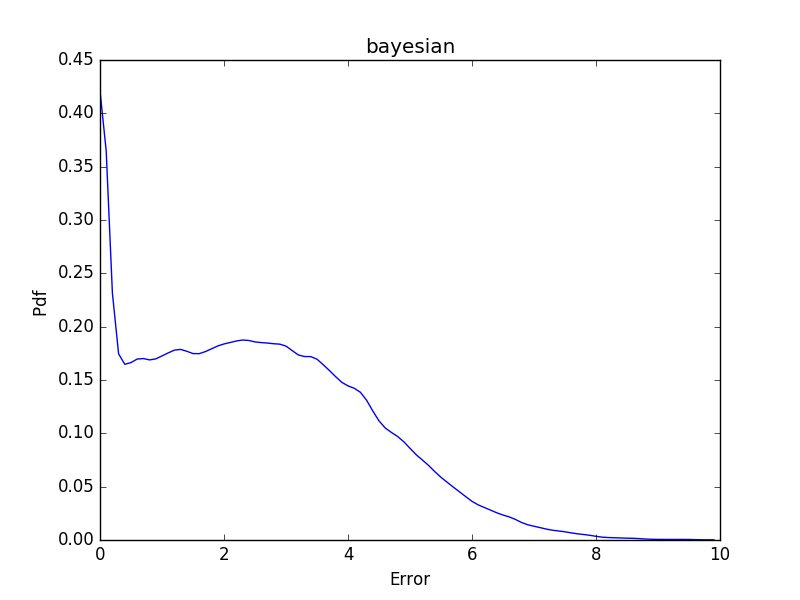
\includegraphics[scale=0.5]{Figures/bayesrtomni.png}
	\caption{This graph shows the approximation probability density function of $|r_{t}-\hat{r_{t}}|$ corresponding to system equipped with isotropic antennas under scheme of \ref{section:BayesEstimation}. }
	\label{figure: BayesRtomni}
\end{figure}
Comparing the PDF curves in Fig.~\ref{figure: BayesRtdir} and Fig.~\ref{figure: BayesRtomni}, the distribution of the error occurs in system with directional antennas appears closer to zero.
This result, along with fact that the BMSE of directional systems is smaller, shows that systems with directional antennas perform better.
This performance improvement results from the directional antennas being more discriminating than the isotropic antennas. 


\subsection{Maximum Likelihood Estimation}

In this section, we look into the maximum likelihood estimation framework mentioned in Section~\ref{section:Maxestimation}.
We use the average mean squared error to evaluate the performance of our estimator.
As before, the total Poisson rates is set to be 32 and the curves are functions of splitting coefficient $\alpha$.
\begin{figure}[]
	\centering
	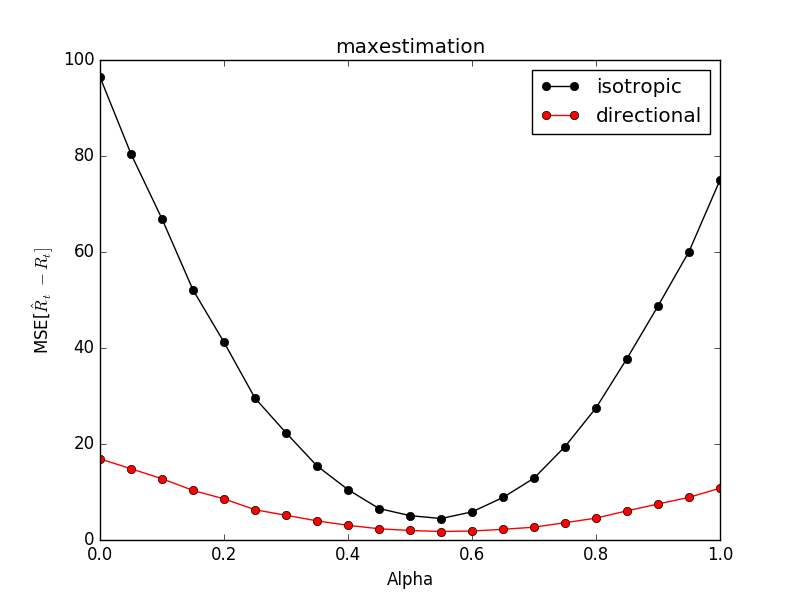
\includegraphics[scale=0.6]{Figures/MaxRt.png}
	\caption{This figure shows mean squared error as functions of splitting parameter under scheme of Section~\ref{section:Maxestimation}. Black line correspond to performance of system equipped with isotropic antennas, whereas red line correspond to the performance of systems with directional antennas. }
	\label{figure: MaxRt}
\end{figure}
The black curve in Fig.~\ref{figure: MaxRt} shows the MSE when the maximum likelihood estimator operates on data collected using isotropic antennas.
The red curve in Fig.~\ref{figure: MaxRt} corresponds to the scenario where the estimator operates on data collected by directional antennas.
The four directional antennas are located at the four corners of the target area, and they are pointing directly towards the center.
These antennas have a 3~dB beam-width of $\theta_{\mathrm{3dB}} = 90^{\circ}$ and a nominal attenuation floor of $G_{\mathrm{floor}} = 20$~dB.
Every point is obtained by averaging over fifty thousand trials.
The MSE is smaller for systems using directional antennas.

The confidence interval of the absolute error $|r_{t}-\hat{r_{t}}|$ corresponding to the isotropic antennas and the directional antennas are summarized in Table~\ref{table:ConfidenceMax}.
\begin{table}[bht]
	\caption{Confidence interval of $|r_{t}-\hat{r_{t}}|$ for simulation corresponding to the Maximum likelihood scheme.} \label{table:ConfidenceMax}
	\centerline{
		\begin{tabular}{|l|l|}
			\hline
			\multicolumn{1}{|c|}{\textbf{Antenna type}} &
			\multicolumn{1}{|c|}{\textbf{Confidence interval}} \\
			\hline
			Directional & $2.080484 \pm 0.002809$ \\
			\hline
			Isotropic & $4.972427 \pm 0.006020$ \\
			\hline
		\end{tabular}}
\end{table}
\begin{figure}[]
	\centering
	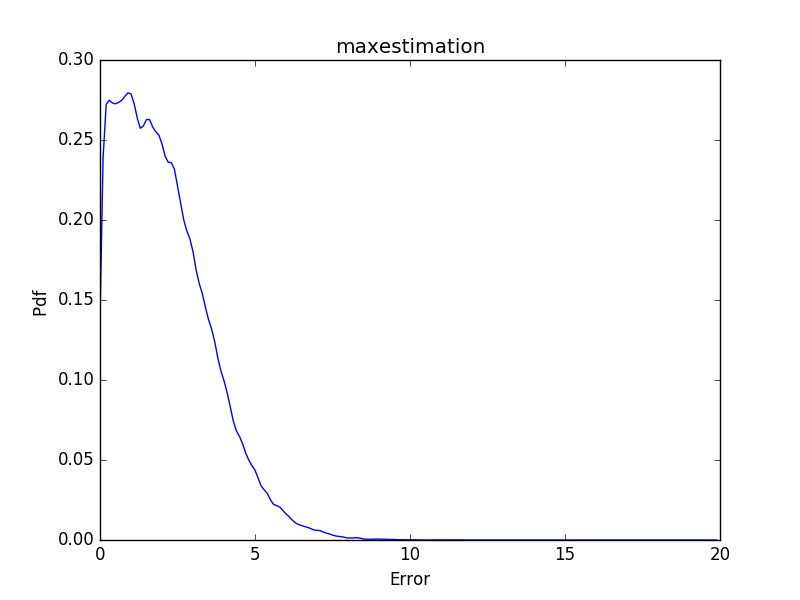
\includegraphics[scale=0.5]{Figures/maxrtdir.png}
	\caption{This graph shows the approximation probability density function of $|r_{t}-\hat{r_{t}}|$ corresponding to system equipped with directional antennas under scheme of \ref{section:Maxestimation}. }
	\label{figure: MaxRtdir}
\end{figure}
\begin{figure}[]
	\centering
	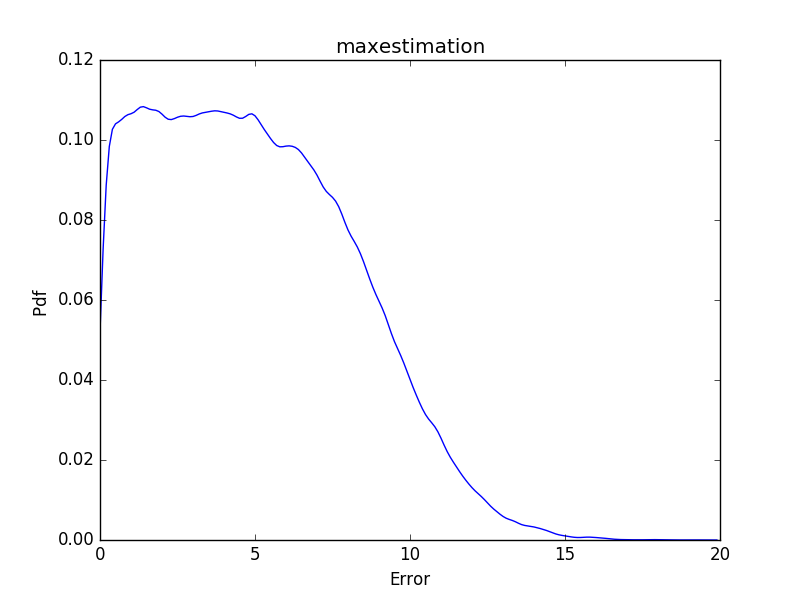
\includegraphics[scale=0.5]{Figures/maxrtomni.png}
	\caption{This graph shows the approximation probability density function of $|r_{t}-\hat{r_{t}}|$ corresponding to system equipped with isotropic antennas under scheme of \ref{section:Maxestimation}. }
	\label{figure: MaxRtomni}
\end{figure}
Compared the PDF curves in Fig.~\ref{figure: MaxRtdir} and Fig.~\ref{figure: MaxRtomni}, we see that the distribution of the error for systems with directional antennas appears closer to zero.
This result, along with the fact that the MSE for the directional systems is smaller, shows that directional antennas outperform isotropic antennas within this context.
Again, these results indicate that the information obtained from the directional antennas is more discriminating than the isotropic antennas. 


